\documentclass[11pt,fleqn]{book} % Default font size and left-justified equations

%%%%%%%%%%%%%%%%%%%%%%%%%%%%%%%%%%%%%%%%%
% The Legrand Orange Book
% Structural Definitions File
% Version 2.1 (26/09/2018)
%
% Original author:
% Mathias Legrand (legrand.mathias@gmail.com) with modifications by:
% Vel (vel@latextemplates.com)
% 
% This file was downloaded from:
% http://www.LaTeXTemplates.com
%
% License:
% CC BY-NC-SA 3.0 (http://creativecommons.org/licenses/by-nc-sa/3.0/)
%
%%%%%%%%%%%%%%%%%%%%%%%%%%%%%%%%%%%%%%%%%

%----------------------------------------------------------------------------------------
%	VARIOUS REQUIRED PACKAGES AND CONFIGURATIONS
%----------------------------------------------------------------------------------------

\usepackage[table]{xcolor}

\usepackage{graphicx}
\usepackage{tabularx} % Required for including pictures
\usepackage{pgf,tikz,tkz-tab,eurosym,yhmath, stmaryrd}
\usepackage{pgfplots}
\usepackage{mathrsfs}
\usetikzlibrary{patterns}
\usetikzlibrary{trees}
\graphicspath{{../../Pictures/}}
\usepackage{multicol} 


\usepackage[english]{babel} % English language/hyphenation
\usepackage{icomma}
\usepackage{enumitem} % Customize lists
\setlist{nolistsep, nosep, nolistsep} % Reduce spacing between bullet points and numbered lists

\usepackage{booktabs} % Required for nicer horizontal rules in tables

 % Required for specifying colors by name


\definecolor{ocre}{RGB}{243,102,25} % Define the orange color used for highlighting throughout the book

\usepackage{listings}

\definecolor{codegreen}{rgb}{0,0.6,0}
\definecolor{codegray}{rgb}{0.5,0.5,0.5}
\definecolor{codepurple}{rgb}{0.58,0,0.82}
\definecolor{backcolour}{rgb}{0.95,0.95,0.92}

\lstdefinestyle{mystyle}{
    backgroundcolor=\color{backcolour},   
    commentstyle=\color{codegreen},
    keywordstyle=\color{magenta},
    numberstyle=\tiny\color{codegray},
    stringstyle=\color{codepurple},
    basicstyle=\ttfamily\footnotesize,
    breakatwhitespace=false,         
    breaklines=true,                 
    captionpos=b,                    
    keepspaces=true,                 
    numbers=left,                    
    numbersep=5pt,                  
    showspaces=false,                
    showstringspaces=false,
    showtabs=false,                  
    tabsize=2
}

\lstset{style=mystyle}

%----------------------------------------------------------------------------------------
% Paramétrage XSIM
%----------------------------------------------------------------------------------------

\usepackage[no-files]{xsim}


\DeclareExerciseEnvironmentTemplate{myex}{%
    \textbf{%
      \hypertarget{ex:\ExerciseID}{\sffamily{\ensuremath{\blacktriangleright}} Exercice \GetExerciseProperty{counter} \GetExerciseProperty{subtitle} --}
      \hyperlink{sol:\ExerciseID}{Voir le corrigé}%
    }\par
}{\par\smallskip}

\DeclareExerciseEnvironmentTemplate{mysol}{%
    \textbf{%
      \hypertarget{sol:\ExerciseID}{\sffamily{\ensuremath{\blacktriangleright}} Correction \GetExerciseProperty{counter} --}
      \hyperlink{ex:\ExerciseID}{Voir l'énoncé}%
    }\par
}{\par\medskip}

\xsimsetup{
  exercise/template = myex ,
  solution/template = mysol 
}

%Collection exercices

\DeclareExerciseTagging{topic}

\xsimsetup{collect}

%----------------------------------------------------------------------------------------
% SYMBOLES
%----------------------------------------------------------------------------------------

\newcommand\imCMsym[4][\mathord]{%
  \DeclareFontFamily{U} {#2}{}
  \DeclareFontShape{U}{#2}{m}{n}{
    <-6> #25
    <6-7> #26
    <7-8> #27
    <8-9> #28
    <9-10> #29
    <10-12> #210
    <12-> #212}{}
  \DeclareSymbolFont{CM#2} {U} {#2}{m}{n}
  \DeclareMathSymbol{#4}{#1}{CM#2}{#3}
}
\newcommand\alsoimCMsym[4][\mathord]{\DeclareMathSymbol{#4}{#1}{CM#2}{#3}}

\imCMsym{cmmi}{124}{\CMjmath}

\newcommand{\Oij}{(O\,;\,\vec{\imath}\,,\, \vec{\CMjmath} )}
\newcommand{\Oijk}{(O\,;\,\vec{\imath}\,,\, \vec{\CMjmath}\,,\,\vec{k})}

\newcommand\e{\mathrm{e}}
\newcommand\R{\mathbb{R}}
\newcommand\N{\mathbb{N}}


%----------------------------------------------------------------------------------------
%	MARGINS
%----------------------------------------------------------------------------------------

\usepackage{geometry} % Required for adjusting page dimensions and margins

\geometry{
	paper=a4paper, % Paper size, change to letterpaper for US letter size
	top=3cm, % Top margin
	bottom=3cm, % Bottom margin
	left=2cm, % Left margin
	right=2cm, % Right margin
	headheight=14pt, % Header height
	footskip=1.4cm, % Space from the bottom margin to the baseline of the footer
	headsep=10pt, % Space from the top margin to the baseline of the header
	%showframe, % Uncomment to show how the type block is set on the page
}

\setlength{\parindent}{0pt}
\parskip=5pt



%----------------------------------------------------------------------------------------
%	FONTS
%----------------------------------------------------------------------------------------

\usepackage{avant} % Use the Avantgarde font for headings
\usepackage{times} % Use the Times font for headings
\usepackage{mathptmx} % Use the Adobe Times Roman as the default text font together with math symbols from the Sym­bol, Chancery and Com­puter Modern fonts

%\usepackage{microtype} % Slightly tweak font spacing for aesthetics
%\usepackage[utf8]{inputenc} % Required for including letters with accents
\usepackage[T1]{fontenc} % Use 8-bit encoding that has 256 glyphs

%----------------------------------------------------------------------------------------
%	BIBLIOGRAPHY AND INDEX
%----------------------------------------------------------------------------------------

\usepackage[style=numeric,citestyle=numeric,sorting=nyt,sortcites=true,autopunct=true,babel=hyphen,hyperref=true,abbreviate=false,backref=true,backend=biber]{biblatex}
\addbibresource{bibliography.bib} % BibTeX bibliography file
\defbibheading{bibempty}{}

\usepackage{calc} % For simpler calculation - used for spacing the index letter headings correctly
\usepackage{makeidx} % Required to make an index
\makeindex % Tells LaTeX to create the files required for indexing

%----------------------------------------------------------------------------------------
%	MAIN TABLE OF CONTENTS
%----------------------------------------------------------------------------------------

\usepackage{titletoc} % Required for manipulating the table of contents

\contentsmargin{0cm} % Removes the default margin

% Part text styling (this is mostly taken care of in the PART HEADINGS section of this file)
\titlecontents{part}
	[0cm] % Left indentation
	{\addvspace{20pt}\bfseries} % Spacing and font options for parts
	{}
	{}
	{}

% Chapter text styling
\titlecontents{chapter}
	[1.25cm] % Left indentation
	{\addvspace{12pt}\large\sffamily\bfseries} % Spacing and font options for chapters
	{\color{ocre!60}\contentslabel[\Large\thecontentslabel]{1.25cm}\color{ocre}} % Formatting of numbered sections of this type
	{\color{ocre}} % Formatting of numberless sections of this type
	{\color{ocre!60}\normalsize\;\titlerule*[.5pc]{.}\;\thecontentspage} % Formatting of the filler to the right of the heading and the page number

% Section text styling
\titlecontents{section}
	[1.25cm] % Left indentation
	{\addvspace{3pt}\sffamily\bfseries} % Spacing and font options for sections
	{\contentslabel[\thecontentslabel]{1.25cm}} % Formatting of numbered sections of this type
	{} % Formatting of numberless sections of this type
	{\hfill\color{black}\thecontentspage} % Formatting of the filler to the right of the heading and the page number

% Subsection text styling
\titlecontents{subsection}
	[1.25cm] % Left indentation
	{\addvspace{1pt}\sffamily\small} % Spacing and font options for subsections
	{\contentslabel[\thecontentslabel]{1.25cm}} % Formatting of numbered sections of this type
	{} % Formatting of numberless sections of this type
	{\ \titlerule*[.5pc]{.}\;\thecontentspage} % Formatting of the filler to the right of the heading and the page number

% Figure text styling
\titlecontents{figure}
	[1.25cm] % Left indentation
	{\addvspace{1pt}\sffamily\small} % Spacing and font options for figures
	{\thecontentslabel\hspace*{1em}} % Formatting of numbered sections of this type
	{} % Formatting of numberless sections of this type
	{\ \titlerule*[.5pc]{.}\;\thecontentspage} % Formatting of the filler to the right of the heading and the page number

% Table text styling
\titlecontents{table}
	[1.25cm] % Left indentation
	{\addvspace{1pt}\sffamily\small} % Spacing and font options for tables
	{\thecontentslabel\hspace*{1em}} % Formatting of numbered sections of this type
	{} % Formatting of numberless sections of this type
	{\ \titlerule*[.5pc]{.}\;\thecontentspage} % Formatting of the filler to the right of the heading and the page number

%----------------------------------------------------------------------------------------
%	MINI TABLE OF CONTENTS IN PART HEADS
%----------------------------------------------------------------------------------------

% Chapter text styling
\titlecontents{lchapter}
	[0em] % Left indentation
	{\addvspace{15pt}\large\sffamily\bfseries} % Spacing and font options for chapters
	{\color{ocre}\contentslabel[\Large\thecontentslabel]{1.25cm}\color{ocre}} % Chapter number
	{}  
	{\color{ocre}\normalsize\sffamily\bfseries\;\titlerule*[.5pc]{.}\;\thecontentspage} % Page number

% Section text styling
\titlecontents{lsection}
	[0em] % Left indentation
	{\sffamily\small} % Spacing and font options for sections
	{\contentslabel[\thecontentslabel]{1.25cm}} % Section number
	{}
	{}

% Subsection text styling (note these aren't shown by default, display them by searchings this file for tocdepth and reading the commented text)
\titlecontents{lsubsection}
	[.5em] % Left indentation
	{\sffamily\footnotesize} % Spacing and font options for subsections
	{\contentslabel[\thecontentslabel]{1.25cm}}
	{}
	{}

%----------------------------------------------------------------------------------------
%	HEADERS AND FOOTERS
%----------------------------------------------------------------------------------------


\usepackage{fancyhdr} % Required for header and footer configuration

\pagestyle{fancy}
\renewcommand{\chaptermark}[1]{\markboth{\sffamily\normalsize\bfseries\ \thechapter.\ #1}{}} % Chapter text font settings
\renewcommand{\sectionmark}[1]{\markright{\sffamily\normalsize\thesection\hspace{5pt}#1}{}} % Section text font settings
\fancyhf{} \fancyhead[LE,RO]{\sffamily\normalsize\thepage} % Font setting for the page number in the header
\fancyhead[LO]{\rightmark} % Print the nearest section name on the left side of odd pages
\fancyhead[RE]{\leftmark} % Print the current chapter name on the right side of even pages

\fancyfoot[L]{Jason LAPEYRONNIE}
\fancyfoot[R]{\href{http://mathoutils.fr}{http://mathoutils.fr}} % Uncomment to include a footer

\renewcommand{\headrulewidth}{0.5pt} % Thickness of the rule under the header
\renewcommand{\footrulewidth}{0.5pt} % Thickness of the rule under the header

\fancypagestyle{plain}{% Style for when a plain pagestyle is specified
	\fancyhead{}\renewcommand{\headrulewidth}{0pt}%
}

% Removes the header from odd empty pages at the end of chapters
\makeatletter
\renewcommand{\cleardoublepage}{
\clearpage\ifodd\c@page\else
\hbox{}
\vspace*{\fill}
\thispagestyle{empty}
\newpage
\fi}

%----------------------------------------------------------------------------------------
%	THEOREM STYLES
%----------------------------------------------------------------------------------------

\usepackage{amsmath,amsfonts,amssymb,amsthm} % For math equations, theorems, symbols, etc

\newcommand{\intoo}[2]{\mathopen{]}#1\,;#2\mathclose{[}}
\newcommand{\ud}{\mathop{\mathrm{{}d}}\mathopen{}}
\newcommand{\intff}[2]{\mathopen{[}#1\,;#2\mathclose{]}}
\renewcommand{\qedsymbol}{$\blacksquare$}
\newtheorem{notation}{Notation}[section]

% Boxed/framed environments
\newtheoremstyle{ocrenumbox}% Theorem style name
{0pt}% Space above
{0pt}% Space below
{\normalfont}% Body font
{}% Indent amount
{\small\bf\sffamily\color{ocre}}% Theorem head font
{\;:\;}% Punctuation after theorem head
{0.25em}% Space after theorem head
{\small\sffamily\color{ocre}\thmname{#1}\nobreakspace\thmnumber{\@ifnotempty{#1}{}\@upn{#2}}% Theorem text (e.g. Theorem 2.1)
\thmnote{\nobreakspace\the\thm@notefont\sffamily\bfseries\color{black}---\nobreakspace#3}} % Optional theorem note

\newtheoremstyle{blacknumex}% Theorem style name
{5pt}% Space above
{10pt}% Space below
{\normalfont}% Body font
{} % Indent amount
{\small\bf\sffamily}% Theorem head font
{\;:\;}% Punctuation after theorem head
{0.25em}% Space after theorem head
{\small\sffamily{\tiny\ensuremath{\blacksquare}}\nobreakspace\thmname{#1}\nobreakspace\thmnumber{\@ifnotempty{#1}{}\@upn{#2}}% Theorem text (e.g. Theorem 2.1)
\thmnote{\nobreakspace\the\thm@notefont\sffamily\bfseries---\nobreakspace#3}}% Optional theorem note

\newtheoremstyle{blacknumexo}% Theorem style name
{15pt}% Space above
{10pt}% Space below
{\normalfont}% Body font
{} % Indent amount
{\small\bf\sffamily}% Theorem head font
{}% Punctuation after theorem head
{0.5em}% Space after theorem head
{\small\sffamily{\ensuremath{\blacktriangleright}}\nobreakspace\thmname{#1}\nobreakspace\thmnumber{\@ifnotempty{#1}{}\@upn{#2}}% Theorem text (e.g. Theorem 2.1)
\thmnote{\nobreakspace\the\thm@notefont\sffamily\bfseries---\nobreakspace#3} \\}% Optional theorem note



\newtheoremstyle{blacknumbox} % Theorem style name
{0pt}% Space above
{5pt}% Space below
{}% Body font
{}% Indent amount
{\large\bf\sffamily}% Theorem head font
{\;:\;}% Punctuation after theorem head
{0.25em}% Space after theorem head
{\small\sffamily\thmname{#1}\nobreakspace\thmnumber{\@ifnotempty{#1}{}\@upn{#2}}% Theorem text (e.g. Theorem 2.1)
\thmnote{\nobreakspace\the\thm@notefont\sffamily\bfseries---\nobreakspace#3}}% Optional theorem note

% Non-boxed/non-framed environments
\newtheoremstyle{ocrenum}% Theorem style name
{5pt}% Space above
{5pt}% Space below
{\normalfont}% Body font
{}% Indent amount
{\small\bf\sffamily\color{ocre}}% Theorem head font
{\;:\;}% Punctuation after theorem head
{0.25em}% Space after theorem head
{\small\sffamily\color{ocre}\thmname{#1}\nobreakspace\thmnumber{\@ifnotempty{#1}{}\@upn{#2}}% Theorem text (e.g. Theorem 2.1)
\thmnote{\nobreakspace\the\thm@notefont\sffamily\bfseries\color{black}---\nobreakspace#3}} % Optional theorem note
\makeatother

% Defines the theorem text style for each type of theorem to one of the three styles above
\newcounter{dummy} 
\newcounter{thm}
\newcounter{correction}
\newcounter{qst}
\theoremstyle{ocrenumbox}
\newtheorem{theoremeT}[dummy]{Théorème}
\newtheorem{exerciseT}{Propriété}
\newtheorem{principeT}{Principe}
\theoremstyle{blacknumex}
\newtheorem{exampleT}{Exemple}
\theoremstyle{blacknumexo}
\newtheorem{exo}[thm]{Exercice}
\newtheorem{corr}[correction]{Correction}
\newtheorem{quest}[qst]{Question}
\theoremstyle{blacknumbox}
\newtheorem{vocabulary}{Vocabulary}[section]
\newtheorem{definitionT}{Définition}
\newtheorem{corollaryT}[dummy]{Corollary}
\theoremstyle{ocrenum}
\newtheorem{proofT}[dummy]{Démonstration}


%----------------------------------------------------------------------------------------
%	DEFINITION OF COLORED BOXES
%----------------------------------------------------------------------------------------

\RequirePackage[framemethod=default]{mdframed} % Required for creating the theorem, definition, exercise and corollary boxes

% Theorem box
\newmdenv[skipabove=7pt,
skipbelow=7pt,
backgroundcolor=black!5,
linecolor=ocre,
innerleftmargin=5pt,
innerrightmargin=5pt,
innertopmargin=10pt,
leftmargin=0cm,
rightmargin=0cm,
innerbottommargin=5pt]{tBox}

%Proposition box	  
\newmdenv[skipabove=7pt,
skipbelow=7pt,
rightline=false,
leftline=true,
topline=false,
bottomline=false,
backgroundcolor=ocre!10,
linecolor=ocre,
innerleftmargin=5pt,
innerrightmargin=5pt,
innertopmargin=10pt,
innerbottommargin=3pt,
leftmargin=0cm,
rightmargin=0cm,
linewidth=4pt]{eBox}	

% Definition box
\newmdenv[skipabove=7pt,
backgroundcolor=ocre!4,
skipbelow=7pt,
rightline=false,
leftline=true,
topline=false,
bottomline=false,
linecolor=ocre,
innerleftmargin=5pt,
innerrightmargin=5pt,
innertopmargin=10pt,
leftmargin=0cm,
rightmargin=0cm,
linewidth=4pt,
innerbottommargin=5pt]{dBox}	

% Corollary box
\newmdenv[skipabove=7pt,
skipbelow=7pt,
rightline=false,
leftline=true,
topline=false,
bottomline=false,
linecolor=gray,
backgroundcolor=black!5,
innerleftmargin=5pt,
innerrightmargin=5pt,
innertopmargin=5pt,
leftmargin=0cm,
rightmargin=0cm,
linewidth=4pt,
innerbottommargin=5pt]{cBox}

\newmdenv[skipabove=7pt,
skipbelow=7pt,
backgroundcolor=black!5,
innerleftmargin=5pt,
topline=false,
bottomline=false,
rightline=false,
leftline=false,
innerrightmargin=5pt,
innertopmargin=5pt,
leftmargin=0cm,
rightmargin=0cm,
innerbottommargin=5pt]{xBox}

% Creates an environment for each type of theorem and assigns it a theorem text style from the "Theorem Styles" section above and a colored box from above
\newenvironment{theorem}{\begin{tBox}\begin{theoremeT}}{\end{theoremeT}\end{tBox}}

\newenvironment{exo2}{\noindent \begin{exo}\item\relax \noindent \begin{eBox}\item\relax}{\end{eBox}\end{exo}}


\newenvironment{proposition}{\begin{eBox}\begin{exerciseT}}{\hfill{\color{ocre}}\end{exerciseT}\end{eBox}}		

\newenvironment{principe}{\begin{eBox}\begin{principeT}}{\hfill{\color{ocre}}\end{principeT}\end{eBox}}	
		  
\newenvironment{definition}{\begin{dBox}\begin{definitionT}}{\end{definitionT}\end{dBox}}	

\newenvironment{example}{\begin{xBox}\begin{exampleT}}{\hfill{\tiny\ensuremath{\blacksquare}}\end{exampleT}\end{xBox}}

\newenvironment{demonstration}{\begin{proofT}}{\hfill{\tiny\ensuremath{\square}}\end{proofT}}		
\newenvironment{corollary}{\begin{cBox}\begin{corollaryT}}{\end{corollaryT}\end{cBox}}	

%----------------------------------------------------------------------------------------
%	REMARK ENVIRONMENT
%----------------------------------------------------------------------------------------

\newenvironment{remark}{\par\vspace{5pt}\small % Vertical white space above the remark and smaller font size
\begin{list}{}{
\leftmargin=25pt % Indentation on the left
\rightmargin=15pt}\item\ignorespaces % Indentation on the right
\makebox[-2.5pt]{\begin{tikzpicture}[overlay]
\node[draw=ocre!60,line width=1pt,circle,fill=ocre!25,font=\sffamily\bfseries,inner sep=2pt,outer sep=0pt] at (-15pt,0pt){\textcolor{ocre}{R}};\end{tikzpicture}} % Orange R in a circle
\advance\baselineskip -1pt}{\end{list}\vskip5pt} % Tighter line spacing and white space after remark

%----------------------------------------------------------------------------------------
%	SECTION NUMBERING IN THE MARGIN
%----------------------------------------------------------------------------------------

\makeatletter
\renewcommand{\@seccntformat}[1]{\llap{\textcolor{ocre}{\csname the#1\endcsname}\hspace{1em}}}                    
\renewcommand{\section}{\@startsection{section}{1}{\z@}
{-4ex \@plus -1ex \@minus -.4ex}
{1ex \@plus.2ex }
{\normalfont\LARGE\sffamily\bfseries}}
\renewcommand{\subsection}{\@startsection {subsection}{2}{\z@}
{-3ex \@plus -0.1ex \@minus -.4ex}
{0.5ex \@plus.2ex }
{\normalfont\sffamily\bfseries}}
\renewcommand{\subsubsection}{\@startsection {subsubsection}{3}{\z@}
{-2ex \@plus -0.1ex \@minus -.2ex}
{.2ex \@plus.2ex }
{\normalfont\small\sffamily\bfseries}}                        
\renewcommand\paragraph{\@startsection{paragraph}{4}{\z@}
{-2ex \@plus-.2ex \@minus .2ex}
{.1ex}
{\normalfont\small\sffamily\bfseries}}

%----------------------------------------------------------------------------------------
%	PART HEADINGS
%----------------------------------------------------------------------------------------

% Numbered part in the table of contents
\newcommand{\@mypartnumtocformat}[2]{%
	\setlength\fboxsep{0pt}%
	\noindent\colorbox{ocre!20}{\strut\parbox[c][.7cm]{\ecart}{\color{ocre!70}\Large\sffamily\bfseries\centering#1}}\hskip\esp\colorbox{ocre!40}{\strut\parbox[c][.7cm]{\linewidth-\ecart-\esp}{\Large\sffamily\centering#2}}%
}

% Unnumbered part in the table of contents
\newcommand{\@myparttocformat}[1]{%
	\setlength\fboxsep{0pt}%
	\noindent\colorbox{ocre!40}{\strut\parbox[c][.7cm]{\linewidth}{\Large\sffamily\centering#1}}%
}

\newlength\esp
\setlength\esp{4pt}
\newlength\ecart
\setlength\ecart{1.2cm-\esp}
\newcommand{\thepartimage}{}%
\newcommand{\partimage}[1]{\renewcommand{\thepartimage}{#1}}%
\def\@part[#1]#2{%
\ifnum \c@secnumdepth >-2\relax%
\refstepcounter{part}%
\addcontentsline{toc}{part}{\texorpdfstring{\protect\@mypartnumtocformat{\thepart}{#1}}{\partname~\thepart\ ---\ #1}}
\else%
\addcontentsline{toc}{part}{\texorpdfstring{\protect\@myparttocformat{#1}}{#1}}%
\fi%
\startcontents%
\markboth{}{}%
{\thispagestyle{empty}%
\begin{tikzpicture}[remember picture,overlay]%
\node at (current page.north west){\begin{tikzpicture}[remember picture,overlay]%	
\fill[ocre!20](0cm,0cm) rectangle (\paperwidth,-\paperheight);
\node[anchor=north] at (4cm,-3.25cm){\color{ocre!40}\fontsize{220}{100}\sffamily\bfseries\thepart}; 
\node[anchor=south east] at (\paperwidth-1cm,-\paperheight+1cm){\parbox[t][][t]{8.5cm}{
\printcontents{l}{0}{\setcounter{tocdepth}{1}}% The depth to which the Part mini table of contents displays headings; 0 for chapters only, 1 for chapters and sections and 2 for chapters, sections and subsections
}};
\node[anchor=north east] at (\paperwidth-1.5cm,-3.25cm){\parbox[t][][t]{15cm}{\strut\raggedleft\color{white}\fontsize{30}{30}\sffamily\bfseries#2}};
\end{tikzpicture}};
\end{tikzpicture}}%
\@endpart}
\def\@spart#1{%
\startcontents%
\phantomsection
{\thispagestyle{empty}%
\begin{tikzpicture}[remember picture,overlay]%
\node at (current page.north west){\begin{tikzpicture}[remember picture,overlay]%	
\fill[ocre!20](0cm,0cm) rectangle (\paperwidth,-\paperheight);
\node[anchor=north east] at (\paperwidth-1.5cm,-3.25cm){\parbox[t][][t]{15cm}{\strut\raggedleft\color{white}\fontsize{30}{30}\sffamily\bfseries#1}};
\end{tikzpicture}};
\end{tikzpicture}}
\addcontentsline{toc}{part}{\texorpdfstring{%
\setlength\fboxsep{0pt}%
\noindent\protect\colorbox{ocre!40}{\strut\protect\parbox[c][.7cm]{\linewidth}{\Large\sffamily\protect\centering #1\quad\mbox{}}}}{#1}}%
\@endpart}
\def\@endpart{\vfil\newpage
\if@twoside
\if@openright
\null
\thispagestyle{empty}%
\newpage
\fi
\fi
\if@tempswa
\twocolumn
\fi}

%----------------------------------------------------------------------------------------
%	CHAPTER HEADINGS
%----------------------------------------------------------------------------------------

% A switch to conditionally include a picture, implemented by Christian Hupfer
\newif\ifusechapterimage
\usechapterimagetrue
\newcommand{\thechapterimage}{}%
\newcommand{\chapterimage}[1]{\ifusechapterimage\renewcommand{\thechapterimage}{#1}\fi}%
\newcommand{\autodot}{.}
\def\@makechapterhead#1{%
{\parindent \z@ \raggedright \normalfont
\ifnum \c@secnumdepth >\m@ne
\if@mainmatter
\begin{tikzpicture}[remember picture,overlay]
\node at (current page.north west)
{\begin{tikzpicture}[remember picture,overlay]
\node[anchor=north west,inner sep=0pt] at (0,0) {\ifusechapterimage\includegraphics[width=\paperwidth]{\thechapterimage}\fi};
\draw[anchor=west] (\Gm@lmargin,-3cm) node [line width=2pt,rounded corners=15pt,draw=ocre,fill=white,fill opacity=0.5,inner sep=15pt]{\strut\makebox[22cm]{}};
\draw[anchor=west] (\Gm@lmargin+.3cm,-3cm) node {\huge\sffamily\bfseries\color{black}\thechapter\autodot~#1\strut};
\end{tikzpicture}};
\end{tikzpicture}
\else
\begin{tikzpicture}[remember picture,overlay]
\node at (current page.north west)
{\begin{tikzpicture}[remember picture,overlay]
\node[anchor=north west,inner sep=0pt] at (0,0) {\ifusechapterimage\includegraphics[width=\paperwidth]{\thechapterimage}\fi};
\draw[anchor=west] (\Gm@lmargin,-3cm) node [line width=2pt,rounded corners=15pt,draw=ocre,fill=white,fill opacity=0.5,inner sep=15pt]{\strut\makebox[22cm]{}};
\draw[anchor=west] (\Gm@lmargin+.3cm,-3cm) node {\huge\sffamily\bfseries\color{black}#1\strut};
\end{tikzpicture}};
\end{tikzpicture}
\fi\fi\par\vspace*{50\p@}}}

%-------------------------------------------

\def\@makeschapterhead#1{%
\begin{tikzpicture}[remember picture,overlay]
\node at (current page.north west)
{\begin{tikzpicture}[remember picture,overlay]
\node[anchor=north west,inner sep=0pt] at (0,0) {\ifusechapterimage\includegraphics[width=\paperwidth]{\thechapterimage}\fi};
\draw[anchor=west] (\Gm@lmargin,-3cm) node [line width=2pt,rounded corners=15pt,draw=ocre,fill=white,fill opacity=0.5,inner sep=15pt]{\strut\makebox[22cm]{}};
\draw[anchor=west] (\Gm@lmargin+.3cm,-3cm) node {\huge\sffamily\bfseries\color{black}#1\strut};
\end{tikzpicture}};
\end{tikzpicture}
\par\vspace*{50\p@}}
\makeatother

%----------------------------------------------------------------------------------------
%	LINKS
%----------------------------------------------------------------------------------------

\usepackage{hyperref}
\hypersetup{hidelinks,backref=true,pagebackref=true,hyperindex=true,colorlinks=false,breaklinks=true,urlcolor=ocre,bookmarks=true,bookmarksopen=false}

\usepackage{bookmark}
\bookmarksetup{
open,
numbered,
addtohook={%
\ifnum\bookmarkget{level}=0 % chapter
\bookmarksetup{bold}%
\fi
\ifnum\bookmarkget{level}=-1 % part
\bookmarksetup{color=ocre,bold}%
\fi
}
}

\renewcommand*\thesection{\arabic{section}}

\newcommand*{\coord}[3]{% 
  \ensuremath{\overrightarrow{#1}\, 
    \begin{pmatrix} 
      #2\\ 
      #3 
    \end{pmatrix}}}
    
  \newcommand*{\coordb}[2]{% 
  \ensuremath{ 
    \begin{pmatrix} 
      #1\\ 
      #2 
    \end{pmatrix}}}

\newcommand*{\coorde}[4]{% 
  \renewcommand{\arraystretch}{1}\ensuremath{\overrightarrow{#1}\, 
    \begin{pmatrix} 
      #2\\ 
      #3 \\
      #4
    \end{pmatrix}}}    
  \newcommand*{\coordbe}[3]{% 
 \renewcommand{\arraystretch}{1} \ensuremath{ 
    \begin{pmatrix} 
      #1\\ 
      #2 \\
      #3
    \end{pmatrix}}}  
    
\newcommand{\Card}{\mathrm{Card}}



\begin{document}

\chapterimage{../../Pictures/background}


\chapter{Cours : Limites de suite}


\section{Limite d'une suite}

\subsection{Limite infinie}

\begin{definition}[Limite infinie]Soit $(u_n)$ une suite réelle. 
\begin{itemize}
\item On dit que $u_n$ tend vers $+\infty$ lorsque $n$ tend vers $+\infty$ si, pour tout réel $A$, l'intervalle $[A ; +\infty [$ contient tous les termes de la suite $(u_n)$ à partir d'un certain rang. Autrement dit, il existe un entier naturel $N$ tel que, pour tout entier $n \geqslant N$, on a $u_n \geqslant A$. On note alors $\displaystyle \lim _{n\to +\infty} u_n = +\infty$.
\item On dit que $u_n$ tend vers $-\infty$ lorsque $n$ tend vers $+\infty$ si, pour tout réel $A$, l'intervalle $] -\infty ; A [$ contient tous les termes de la suite $(u_n)$ à partir d'un certain rang. Autrement dit, il existe un entier naturel $N$ tel que, pour tout entier $n \geqslant N$, on a $u_n \leqslant A$. On note alors $\displaystyle \lim _{n\to +\infty} u_n = -\infty$.\end{itemize}\end{definition}

La première définition traduit le fait que la suite dépasse n'importe quel seuil donné sans jamais repasser en dessous par la suite. Attention, cela ne signifie pas que les termes de la suite sont de plus en plus grands ; une suite qui tend vers $+\infty$ n'est pas nécessairement croissante.


\textbf{Illustration :} On a représenté graphiquement une certaine suite $(u_n)$ ci-dessous. On se fixe un seuil $A=6$.
\begin{center}
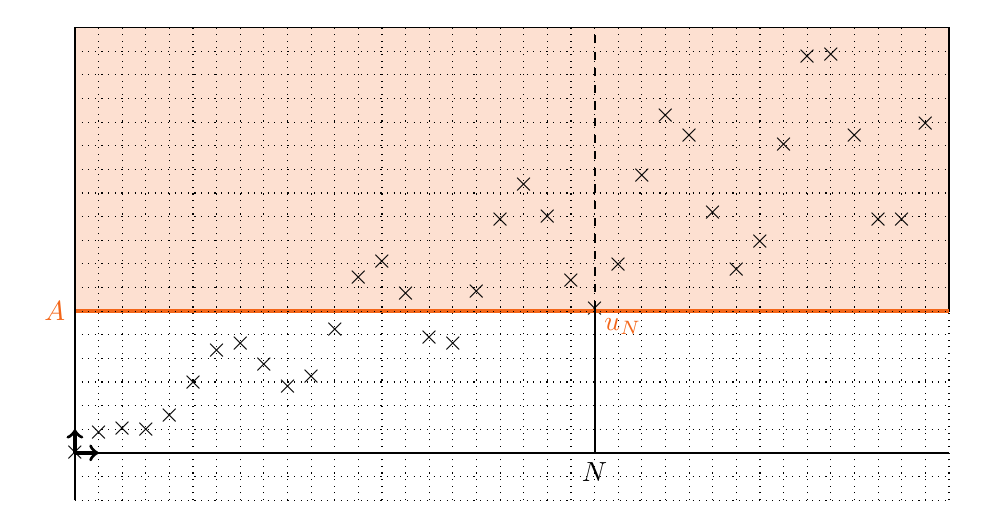
\begin{tikzpicture}[scale=0.3]
\clip (-2,-2) rectangle (38,18);
\draw [fill=ocre!20] (0,6) -- (37,6) -- (37,18) -- (0,18) -- cycle;
\foreach \k in {0,1,...,36} {\draw (\k,{\k^(6/8)*(1.5+cos(deg(\k)))/3+\k/5}) node {$\times$};}

\draw [very thick, ocre, domain = 0:37] plot (\x,6);
\draw [thick] (22,{22^(6/8)*(1.5+cos(deg(22)))/3+22/5}) -- (22,0);
\draw [thick, dashed] (22,{22^(6/8)*(1.5+cos(deg(22)))/3+22/5}) -- (22,18);
\draw [ocre] (22,{22^(6/8)*(1.5+cos(deg(22)))/3+22/5}) node[below right] {$u_{N}$};
\draw  [ocre](0,6) node[left] {$A$};
\draw  (22,0) node[below] {$N$};
\draw [ thin, dotted] (0,-2) grid (37,28);
\draw [thick] (0,0)--(37,0);
\draw [thick] (0,-2)--(0,28);
\draw [->, very thick] (0,0)--(1,0);
\draw [->,very thick] (0,0)--(0,1);

\end{tikzpicture}

\end{center}

On remarque que $u_{12} \geqslant 6$. Cependant, certains des termes suivants sont inférieurs à 6 : pour qu'une suite tende vers $+\infty$, il faut que \textbf{tous les termes} à partir d'un certain rang soient au-dessus du seuil $A$, et ce, peu importe le seuil $A$.
On voit ainsi que, pour tout $n\geqslant 22$, il semblerait qu'on ait bien $u_n \geqslant 6$.

Le raisonnement que nous venons de tenir pour $A=6$ tient pour toutes les valeurs de $A$, aussi grandes soient-elles : la suite $(u_n)$ tend vers $+\infty$.

Naturellement, plus la valeur de $A$ est grande, plus la valeur à partir de laquelle tous les termes de la suite sont tous plus grands que $A$ sera lointaine.

Il faut par ailleurs remarquer et insister \textbf{lourdement} sur le fait qu'une suite qui tend vers $+\infty$ n'est pas forcément croissante. Cette suite ici représentée en est un exemple. Il est également faux de dire qu'une suite qui est strictement croissante tend forcément vers $+\infty$.

\newpage

\begin{example} Pour tout $n$, on pose $u_n=n^2$. $u_n$ tend vers $+\infty$ lorsque $n$ tend vers $+\infty$. 

\vskip80pt
\end{example}

Il y a une différence entre une suite qui tend vers $+\infty$ et une suite non majorée. : évidemment, toute suite qui tend vers $+\infty$ n'est pas majorée, puisque pour tout réel $A$, il y a des termes de la suite supérieurs à $A$.

La réciproque est en revanche fausse sans davantage d'hypothèse sur la suite. Considérons par exemple la suite $(u_n)$ définie pour tout entier naturel $n$ par $u_n=(1+(-1)^n) \, n$. La suite $(u_n)$ n'est pas majorée : elle a des termes arbitrairement grands. Cependant, elle ne tend pas non plus vers $+\infty$ puisqu'un terme sur deux de cette suite vaut 0. Elle ne reste donc pas supérieure à n'importe quel réel donné à partir d'un certain rang (elle est en particulier en dessous de 1 tous les termes impairs).

\subsection{Limite finie : suite convergente}

\begin{definition}Soit $(u_n)$ une suite réelle et $\ell$ un réel. 

On dit que $u_n$ tend vers $\ell$ lorsque $n$ tend vers $+\infty$ si, pour tout $\varepsilon >0$, l'intervalle $] \ell- \varepsilon, \ell+\varepsilon [$ contient tous les termes de la suite $(u_n)$ à partir d'un certain rang.

Autrement dit, pour tout $\varepsilon >0$, il existe un entier $N$ tel que, dès que $n\geqslant N$, on a $|u_n- \ell | \leqslant \varepsilon$.\end{definition}

\textbf{Illustration :} On a représenté graphiquement une certaine suite $(u_n)$ ci-dessous. \begin{center}

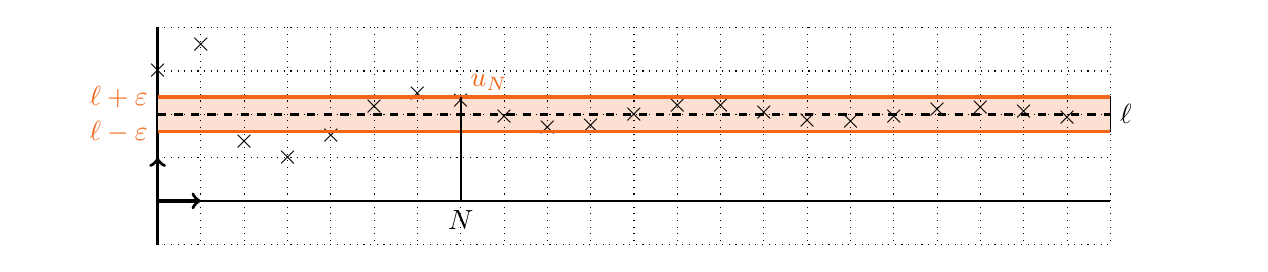
\begin{tikzpicture}[scale=0.55]
\clip (-3,-1) rectangle (25,4);
\draw [thick] (0,0)--(22,0);
\draw [thick] (0,-2)--(0,28);
\draw [->, very thick] (0,0)--(1,0);
\draw [->,very thick] (0,0)--(0,1);

\draw [fill=ocre!20] (0,1.6) -- (22,1.6) -- (22,2.4) -- (0,2.4) -- cycle;
\foreach \k in {1,2,...,21} {\draw (\k,{2+3*cos(deg(\k))/\k}) node {$\times$};}
\draw (0,3) node {$\times$};
\draw [ thin, dotted] (0,-2) grid (22,28);
\draw [very thick, ocre, domain = 0:22] plot (\x,1.6);
\draw [very thick, ocre, domain = 0:22] plot (\x,2.4);
\draw [very thick, dashed, domain = 0:22] plot (\x,2);

\draw [thick] (7,{2+3*cos(deg(7))/7}) -- (7,0);
\draw [thick, dashed] (7,{2+3*cos(deg(7))/7}) -- (7,2.4);
\draw [ocre] (7,{2+3*cos(deg(7))/7}) node[above right] {$u_{N}$};
\draw  [ocre](0,1.6) node[left] {$\ell-\varepsilon$};
\draw  [ocre](0,2.4) node[ left] {$\ell+\varepsilon$};
\draw  (22,2) node[right] {$\ell$};
\draw  (7,0) node[below] {$N$};



\end{tikzpicture}
\end{center}

La suite $(u_n)$ semble tendre vers 2. Par exemple, pour $\varepsilon = 0,4$, tous les termes de la suite sont dans l'intervalle $]2-\varepsilon ; 2+\varepsilon[$, soit $]1,6\,;\, 2,4[$ à partir du rang 7. Ce raisonnement vaut pour n'importe quel $\varepsilon$, aussi petit soit-il.


\begin{proposition}
Soit $(u_n)$ une suite réelle, $\ell$ et $\ell'$ deux réels. Si $u_n$ tend vers $\ell$ et $u_n$ tend vers $\ell'$ lorsque $n$ tend vers $+\infty$, alors $\ell=\ell'$.\end{proposition}

L'idée de la démonstration suivante est assez simple : elle consiste à montrer l'impossibilité d'être à la fois très proche de $\ell$ et de $\ell'$ si ces deux valeurs sont différentes. Pour cela, on va trouver une valeur de $\varepsilon$ pour lesquels les intervalles $] \ell- \varepsilon, \ell+\varepsilon [$ et $] \ell'- \varepsilon, \ell'+\varepsilon [$ sont disjoints, ce qui contredira le fait que ces deux intervalles doivent tous deux contenir tous les termes de la suite à partir d'un certain rang.

\begin{center}
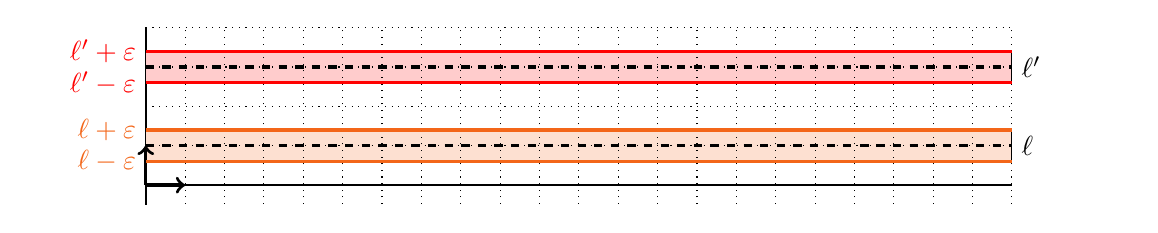
\begin{tikzpicture}[scale=0.5]
\clip (-3,-0.5) rectangle (25,4);
\draw [thick] (0,0)--(22,0);
\draw [thick] (0,-2)--(0,28);


\draw [fill=ocre!20] (0,0.6) -- (22,0.6) -- (22,1.4) -- (0,1.4) -- cycle;
\draw [fill=red!20] (0,2.6) -- (22,2.6) -- (22,3.4) -- (0,3.4) -- cycle;
\draw [->, very thick] (0,0)--(1,0);
\draw [->,very thick] (0,0)--(0,1);

\draw [ thin, dotted] (0,-2) grid (22,28);

\draw [very thick, ocre, domain = 0:22] plot (\x,0.6);
\draw [very thick, ocre, domain = 0:22] plot (\x,1.4);
\draw [very thick, dashed, domain = 0:22] plot (\x,1);

\draw  [ocre](0,0.6) node[left] {$\ell-\varepsilon$};
\draw  [ocre](0,1.4) node[ left] {$\ell+\varepsilon$};
\draw  (22,1) node[right] {$\ell$};


\draw [very thick, red, domain = 0:22] plot (\x,2.6);
\draw [very thick, red, domain = 0:22] plot (\x,3.4);
\draw [very thick, dashed, domain = 0:22] plot (\x,3);

\draw  [red](0,2.6) node[left] {$\ell'-\varepsilon$};
\draw  [red](0,3.4) node[ left] {$\ell'+\varepsilon$};
\draw  (22,3) node[right] {$\ell'$};
\end{tikzpicture}
\end{center}

\begin{demonstration}Supposons que $\ell \neq \ell'$, par exemple que $\ell>\ell'$. Soit $\varepsilon$ un réel strictement positif.
\begin{itemize}
\item Puisque $u_n$ tend vers $\ell$ en $+\infty$, l'intervalle $] \ell- \varepsilon, \ell+\varepsilon [$ contient tous les termes de la suite à partir d'un certain rang $N$. En particulier, à partir d'un certain rang $N$, tous les termes de la suite sont strictement supérieurs à $\ell-\varepsilon $ \item Puisque $u_n$ tend vers $\ell'$ en $+\infty$, l'intervalle $] \ell'- \varepsilon, \ell'+\varepsilon [$ contient tous les termes de la suite à partir d'un certain rang. En particulier, à partir d'un certain rang $N'$, tous les termes de la suite sont strictement inférieurs à $\ell'+\varepsilon $
\end{itemize}
Ainsi, à partir de la plus grande valeur entre $N$ et $N'$, les termes de la suite sont à la fois strictement supérieurs à $\ell-\varepsilon$ et strictement inférieurs à $\ell'+\varepsilon$. Autrement dit, pour tout entier $n \geqslant \max(N,N')$, on a $ \ell-\varepsilon < u_n < \ell'+\varepsilon$.

 Puisque cela vaut pour n'importe quelle valeur de $\varepsilon$, cela reste vrai en prenant par exemple $\varepsilon = \dfrac{\ell-\ell'}{2}$ (ce réel est bien strictement positif puisque $\ell>\ell'$).

Ainsi, pour tout entier $n\geqslant \max(N,N')$, on a $\ell-\dfrac{\ell-\ell'}{2}< u_n < \ell'+\dfrac{\ell-\ell'}{2}$ et donc $\dfrac{\ell+\ell'}{2} < u_n < \dfrac{\ell+\ell'}{2}$ et en particulier $\dfrac{\ell+\ell'}{2} < \dfrac{\ell+\ell'}{2}$. C'est impossible : notre supposition de départ, qui était que $\ell \neq \ell'$ était donc erroné. Par conséquent, on a $\ell=\ell'$.

Le raisonnement que nous venons d'appliquer, qui consiste, en supposant une proposition vraie, à aboutir à une conclusion fausse et à en déduire que la proposition de départ devait donc également être fausse s'appelle le \textbf{raisonnement par l'absurde}.\end{demonstration}


Cette propriété nous permet de définir sans ambiguïté la notion de limite d'une suite.

\begin{definition}[Limite finie, suite convergente] Soit $(u_n)$ une suite réelle et $\ell$ un réel. 

Si $u_n$ tend vers $\ell$ lorsque $n$ tend vers $+\infty$, on dit que $\ell$ est \textbf{LA} \textit{limite} de la suite $(u_n)$ lorsque $n$ tend vers $+\infty$. On note alors $\displaystyle \lim _{ n \to +\infty} u_n = \ell$.


Une suite qui admet une limite finie est dite \textit{convergente}. 

Dans le cas contraire, on parle de suite \textit{divergente} : cela regroupe les suites qui ont une limite infinie mais aussi les suites qui n'admettent pas de limite.\end{definition}



\begin{example} Pour tout entier naturel $n$, on pose $u_n=\dfrac{2n+1}{4n+5}$. \\
Pour se faire une idée de la limite, il est possible de calculer quelques termes de la suite. 

\vskip50pt
Pour le prouver formellement, repassons pas la définition  : pour n'importe quel $\varepsilon >0$, il faut trouver un rang $N$ à partir duquel, pour tout $n>N$, on ait $u_n \in \left] \dfrac{1}{2}-\varepsilon ; \dfrac{1}{2}+\varepsilon \right[$.

Soit $n\in\mathbb{N}$, 
\[u_n-\dfrac{1}{2}=\]
Cette quantité est négative. On a alors \[\left\lvert u_n - \dfrac{1}{2} \right\rvert = \]

Fixons alors $\varepsilon >0$. Ainsi, 
\[ \left\lvert u_n - \dfrac{1}{2} \right\rvert < \varepsilon \Leftrightarrow \]
Ainsi, pour tout $\varepsilon >0$, dès que $n  > \qquad\qquad\qquad $, on a $u_n \in \left] \dfrac{1}{2}-\varepsilon ; \dfrac{1}{2}+\varepsilon \right[$. 

La suite $(u_n)$ est bien convergente et sa limite vaut $\dfrac{1}{2}$.

Par exemple, si $\varepsilon = 0.001$, on a $\dfrac{3}{8\varepsilon}-\dfrac{5}{4}= 374.99$. 

Ainsi, pour tout entier $n\geqslant 375$, on a  $0.499 \leqslant u_n \leqslant 0.501$.\end{example}

Nous verrons très bientôt des résultats qui nous permettront de passer outre cet aspect formel. Même si une telle démonstration de la convergence d'une suite n'est que rarement demandée en classe de terminale, comprendre les bases de ce raisonnement constituera un avantage certain dans les études supérieures.

\begin{proposition}Si une suite est convergente, elle est bornée. Par contraposée, si une suite n'est pas bornée, elle ne peut être convergente.\end{proposition}

 La réciproque est fausse : toute suite bornée n'est pas convergente. 
 
Par exemple, pour tout $n$, prenons $u_n=(-1)^n$. La suite $(u_n)$ est bornée puisque, pour tout $n$, $-1 \leqslant u_n \leqslant 1$. En revanche, elle n'est pas convergente : ses termes de rangs pairs valent tous $1$ et ses termes de rangs impairs valent tous $-1$. Une limite étant unique, la suite $(u_n)$ ne peut être convergente.

\subsection{Limites de suites usuelles}

\begin{proposition} Les limites suivantes sont à connaître.
\begin{center}
\begin{tabularx}{0.9\linewidth}{XXX}
 $\displaystyle \lim _{n\to+\infty} n = $ & $\displaystyle \lim _{n\to+\infty} n^{2} = $ &  $\displaystyle \lim _{n\to+\infty} \dfrac{1}{n} = $ \end{tabularx}
\end{center}

Plus généralement, pour tout entier naturel non nul $\alpha$, $\displaystyle \lim _{n\to+\infty} n^{\alpha} = \qquad\qquad $ et $\displaystyle \lim _{n\to+\infty} \dfrac{1}{n^{\alpha}} = \qquad\qquad$.
\begin{center}
\begin{tabularx}{0.9\linewidth}{XXX}
  $\displaystyle \lim _{n\to+\infty} \sqrt{n} = $ & $\displaystyle \lim _{n\to+\infty} \e^n = $ & $\displaystyle \lim _{n\to+\infty} \e^{-n} = $\end{tabularx}
\end{center}

 Les suites $(\cos(n))$, $(\sin(n))$ et $((-1)^n)$ n'admettent quant à elles pas de limite lorsque $n$ tend vers $+\infty$.
\end{proposition}

\newpage
\section{Opérations sur les limites}

\subsection{Limite de la somme}

\begin{proposition}On considère deux suites réelles $(u_n)$ et $(v_n)$ et deux réels $\ell_1$ et $\ell_2$. 

\begin{tabularx}{\linewidth}{|l|X|X|X|X|X|X|}
\hline
$\displaystyle \lim_{n \to +\infty} u_n$ & $\ell_1$ & $\ell_1$ & $\ell_1$ & $+\infty$ & $-\infty$ & $+\infty$\\
\hline
$\displaystyle \lim_{n \to +\infty} v_n$ & $\ell_2$ & $+\infty$ & $-\infty$ & $+\infty$ & $-\infty$ & $-\infty$\\
\hline
$\displaystyle \lim_{n \to +\infty} (u_n + v_n)$ & $ $ & $ $ & $ $ & $ $ & $ $ & \\
\hline
\end{tabularx}\end{proposition}

\begin{demonstration}Bien qu'elles ne soient pas explicitement au programme, les démonstrations de ces résultats permettent de manipuler et comprendre les définitions des différentes limites de suite. 

On s'intéresse ici au cas où $\displaystyle\lim_{n \to + \infty}u_n=+\infty$ et $\displaystyle \lim_{n \to+\infty}v_n=+\infty$. Les autres démonstrations pourront être traitées en guise d'exercice.

\vskip110pt

\end{demonstration}

\begin{example}Pour tout entier naturel $n$, on pose $u_n=n^2+\e^{-n}-4$. 

\vskip30pt \end{example}

Les cas où $\displaystyle \lim_{n \to +\infty} u_n = +\infty$ et $\displaystyle \lim_{n \to +\infty} v_n = -\infty$ n'obéissent à aucune règle précise : il faut les traiter séparément. L'expression "Forme indéterminée" ne signifie pas qu'il est impossible de déterminer une éventuelle limite : il précise simplement qu'il nous est impossible d'appliquer directement les règles de calcul sur les limites de suite. 

La limite de la somme peut alors aussi bien être 0, 1, $+\infty$, $-\infty$ ou peut même ne pas exister du tout !

\begin{example} Pour tout entier naturel $n$, on pose $u_n = n$, $v_n = 1-n$ et $w_n=n^2+n$.

On a alors $\displaystyle \lim_{n \to +\infty} u_n = \qquad\qquad$ et $\displaystyle \lim_{n \to +\infty} v_n = \qquad\qquad$. 

Il n'est pas possible de conclure sur l'éventuelle limite de la suite $(u_n+v_n)$ avec ces seules informations.

Or, pour tout entier naturel $n$, $u_n+v_n=\qquad\qquad$ et on en déduit que $\displaystyle \lim_{n \to +\infty} (u_n+v_n) = \qquad\qquad$.

Par ailleurs, $\displaystyle \lim_{n \to +\infty} w_n = \qquad\qquad$ et $\displaystyle \lim_{n \to +\infty} v_n = \qquad\qquad$. 

Là encore, il n'est pas possible de conclure sur l'éventuelle limite de la suite $(v_n+w_n)$ avec ces seules informations.

Or, pour tout entier naturel $n$, $v_n+w_n=\qquad\qquad$. Ainsi, $\displaystyle \lim_{n \to +\infty} (v_n+w_n) = \qquad\qquad$. 

Nous avons là deux exemples où la somme de limites "$\infty - \infty $" produit des résultats totalement différents.\end{example}

\newpage

\subsection{Limite du produit}



\begin{proposition}On considère deux suites réelles $(u_n)$ et $(v_n)$ et deux réels $\ell_1$ et $\ell_2$. 
\vskip10pt
\begin{tabularx}{\linewidth}{|l|X|X|X|X|}
\hline
$\displaystyle \lim_{n \to +\infty} u_n$ & $\ell_1 $ & $\ell_1 \neq 0$ &  $\infty$ & $0$ \\
\hline
$\displaystyle \lim_{n \to +\infty} v_n$ & $\ell_2$ & $\infty$  & $\infty$  & $\infty$ \\
\hline
$\displaystyle \lim_{n \to +\infty} (u_n \, v_n)$ &  &   &  &  \\
\hline
\end{tabularx}

\begin{center}
 \textbf{r.s. : Règle des signes}
 \end{center} \vspace{-1cm} \end{proposition}

\begin{example} Pour tout entier naturel non nul $n$, on pose $u_n = \left(\dfrac{3}{n}-4\right)\times (n^2+2\sqrt{n})$.

\vskip80pt

\end{example}

\begin{example} Pour tout entier naturel non nul $n$, on pose $u_n=\dfrac{2}{n}$, $v_n=n$ et $w_n=n^2$. 
\begin{itemize}
\item On a $\displaystyle \lim_{n \to +\infty} u_n = \qquad\qquad$, $\displaystyle \lim_{n \to +\infty} v_n = \qquad\qquad$. Par ailleurs, pour tout entier naturel non nul $n$, $u_n \, v_n = \qquad\qquad$. Ainsi, $\displaystyle \lim_{n \to +\infty} (u_n \, v_n) = \qquad\qquad$.
\vskip5pt
\item On a $\displaystyle \lim_{n \to +\infty} u_n = \qquad\qquad$, $\displaystyle \lim_{n \to +\infty} w_n = \qquad\qquad$. Par ailleurs, pour tout entier naturel non nul $n$, $u_n \, w_n = \qquad\qquad$. Ainsi, $\displaystyle \lim_{n \to +\infty} (u_n \, v_n) = \qquad\qquad$.
\end{itemize} 
On voit sur cet exemple que le produit d'une limite infinie et d'une limite qui vaut 0 peut aboutir à plusieurs résultats différents.\end{example}



\subsection{Limite du quotient}


\begin{definition}Soit $(u_n)$ une suite réelle et $a$ un réel. 

\begin{itemize}
\item On note $\displaystyle\lim_{n \to +\infty}u_n = a^+$ si $u_n$ tend vers $a$ lorsque $n$ tend vers $+\infty$ ET s'il existe un entier $N$ tel que, pour tout entier naturel $n$ supérieur à $N$, on a $u_n \geqslant a$.
\item On note $\displaystyle\lim_{n \to +\infty}u_n = a^-$ si $u_n$ tend vers $a$ lorsque $n$ tend vers $+\infty$ ET s'il existe un entier $N$ tel que, pour tout entier naturel $n$ supérieur à $N$, on a $u_n \leqslant a$.\end{itemize}
\end{definition}

\begin{example}On sait que $\displaystyle\lim_{n \to + \infty}\left(1-\dfrac{1}{n}\right)=1$. Or, pour tout entier naturel non nul $n$, $1-\dfrac{1}{n}\leqslant 1$. 

On pourra alors écrire $\displaystyle\lim_{n \to + \infty}\left(1-\dfrac{1}{n}\right)=1^-$.\end{example}

Cette petite subtilité nous est notamment utile lorsque l'on étudie la limite de quotients dans certains cas...


\begin{proposition}On considère deux suites réelles $(u_n)$ et $(v_n)$ telles que $(v_n)$ ne s'annule pas à partir d'un certain rang. On considère deux réels $l_1$ et $l_2$, avec $l_2 \neq 0$. 
\vskip10pt
\begin{tabularx}{\linewidth}{|l|X|X|X|X|c|c|}
\hline
$\displaystyle \lim_{n \to +\infty} u_n$ & $\ell_1 $ & $\ell_1$ & $\ell_1 \neq 0$ & $\infty$  & $0$ & $\infty$\\
\hline
$\displaystyle \lim_{n \to +\infty} v_n$ & $\ell_2 \neq 0$ & $\infty$ &  $0^+$ ou $0^-$ &  $l_2$, $0^+$ ou $0^-$ & $0$ & $\infty$ \\
\hline
$\displaystyle \lim_{n \to +\infty} \left(\dfrac{u_n}{ v_n}\right)$ &  &  &   &  & \multicolumn{2}{|c|}{ } \\
\hline\end{tabularx}


\begin{center}
 \textbf{r.s. : Règle des signes}\\
 \end{center} 
 \vspace{-1cm}\end{proposition}
 
\begin{example} Pour tout entier naturel non nul $n$ on pose $u_n=\dfrac{1+\frac{2}{n}}{3+n}$.

\vskip40pt \end{example}


\begin{example} Pour tout entier naturel non nul $n$ on pose $u_n=\dfrac{1-n}{\e^{-n}+\frac{1}{n}}$.

\vskip40pt
\end{example}




\section{Formes indéterminées}

\subsection{Factorisation par le terme dominant}

\begin{example} Pour tout entier naturel $n$, on pose $u_n=4n^2+2n+3$ et $v_n = 3n^2+7n-1$. 

On cherche à déterminer $\displaystyle \lim_{n \to +\infty} \dfrac{u_n}{v_n}$. Or, en utilisant les règles sur les calculs de limites, on trouve que $\displaystyle \lim_{n \to +\infty} u_n = +\infty$ et $\displaystyle \lim_{n \to +\infty} v_n = +\infty$. On se retrouve dans le cas "$\dfrac{\infty}{\infty}$".

Il est toutefois possible de factoriser $u_n$ et $v_n$ par leur terme de plus haut degré (ici, $n^2$ dans les deux cas). 

\vskip150pt

\end{example}

Il est à noter qu'avant de se lancer dans la factorisation par le terme dominant, il faut s'assurer que celle-ci est nécessaire : en voulant lever une forme indéterminée inexistante, on peut très vite se retrouver à en créer une involontairement.

\subsection{Quantité conjuguée}

La partie suivante s'intéresse aux formes indéterminées faisant intervenir des racines carrées.

\begin{proposition}Soit $(u_n)$ une suite réelle positive et $a$ un réel positif.
\begin{itemize}
\item Si $\displaystyle \lim_{n \to +\infty} u_n=a$, alors $\displaystyle \lim_{n \to +\infty} \sqrt{u_n}=\sqrt{a}$.
\item Si $\displaystyle \lim_{n \to +\infty} u_n=+\infty$, alors $\displaystyle \lim_{n \to +\infty} \sqrt{u_n}=+\infty$.
\end{itemize}\end{proposition}

\begin{example}Pour tout entier naturel non nul $n$, on pose $u_n = \dfrac{\sqrt{4n^2+1}}{n}$.

\vskip150pt

\end{example}

Lorsque l'on est en présence d'une différence de racines carrées $\sqrt{a}-\sqrt{b}$, on peut multiplier et diviser par la quantité conjuguée $\sqrt{a}+\sqrt{b}$.

L'objectif est ici d'utiliser l'identité remarquable $(x-y)(x+y)=x^2-y^2$. En particulier, dans le cas des racines carrées, cela entraîne que, pour tous réels strictement positifs $a$ et $b$,\[(\sqrt{a}-\sqrt{b})(\sqrt{a}+\sqrt{b})=\sqrt{a}^2-\sqrt{b}^2=a-b.\]

\begin{example} Pour tout entier naturel non nul $n$, on note $u_n=\sqrt{n+1}-\sqrt{n-1}$. Il s'agit de la différence de deux termes qui tendent vers $+\infty$, il n'est pas possible de conclure directement sur sa limite. 
\vskip80pt
\end{example}

\newpage







\end{document}